%%%%% Single page layout:
%%%%% ----------------------------------------------------
\documentclass[12pt,a4paper,paper=a4,oneside,titlepage,pdftex]{scrartcl} 

%%% Additional useful packages
%%% ----------------------------------------------------------------
\usepackage{amsmath,amssymb,amsfonts}
\usepackage{algorithmic}
\usepackage{graphicx}
\usepackage{listings}                
\usepackage{graphicx}
\usepackage{subcaption}
\usepackage{float}
\usepackage[utf8]{inputenc}
\usepackage{booktabs}
\usepackage{pdfpages}
\usepackage{hyperref}
\usepackage{url}
\usepackage{color} %red, green, blue, yellow, cyan, magenta, black, white
\usepackage{lipsum}

\begin{document}
	
\pagenumbering{arabic}

\title{Project Report: Users' satisfaction about Dalarna University's Homepage}
\subtitle{ST3012 Data Collection}
\author{
	\bfseries\Large Authors: Péter Tempfli, Tobias Weiß\\
	\{v19pette, v18tobwe\}@du.se
	\\ \\
	
\includegraphics[]{figures/du-logo.jpg}\\
}

\maketitle
\tableofcontents
\newpage

\section{Abstract}
We write as very last thing
\vspace{10px}
\textbf{Keywords: foo bar}

\section{Introduction}
We write as last thing

\section{Research Question - Tobias}
Users' satisfaction is a very broad topic and the scope has to be narrowed down carefully. A survey about general satisfaction would be doomed to fail. It either would be too big and comprehensive or too general and vague. Both would lead to missing and/or imprecise information.

Therefore, this project focuses on functionality aspects of the "search personal" page. Following main questions were raised:
\begin{enumerate}
	\item If "find personal" is accessed, then the path is intuitive and quick?
	\item If "find personal" page is visited, then the required data is found quickly?
	\item If "find personal" page is visited, then a up-to-date front-end is displayed?
\end{enumerate}

In oder to answer these questions a survey among the website users is conducted.

\section{Methodology}
bla

\subsection{Research design}
General desciption, why do we choose online form? Sequencial sampling, etc.

\subsubsection{Population - Tobias}
What is the population -> logs -> assumptions

\subsubsection{Sampling size - Tobias}
Determin n

\subsubsection{Statistical Indicators}
About the Statistical methods we apply. Here go the dummy tables

\subsubsection{Data Quality Assurance}
Why we use the DESAP checklist

\subsubsection{Data collection plan}
Why (only) a online survey. Why online?

%\begin{figure}[H]
%    \centering
%    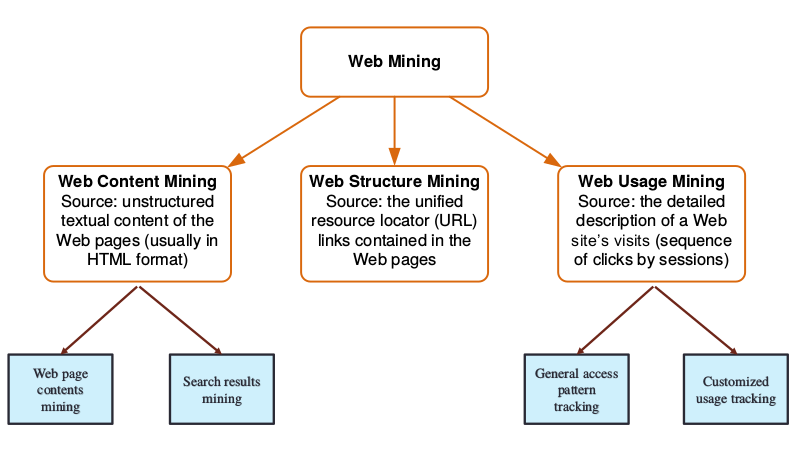
\includegraphics[width=0.7\textwidth]{figures/typed-of-webmining.png}
%    \caption{dummy}
%    \label{fig:XXX}
%\end{figure}

\subsubsection{Ethical considerations}
How do we store the data? What is the problem with Google forms. (Maybe write that in a real research we would use our own form/tool!)

\subsubsection{Legal considerations}
GDPR checkbox in the survery

\subsubsection{Applied tools}
About google forms and R, maybe

\section{Analysis}

\subsection{Pilot}

\subsection{Absolute and Relative Frequencies}

\subsection{(Co-)variances}

\subsection{Independence}

\section{Conclusion}

\section*{References}
\bibliographystyle{ieeetr}
\renewcommand\refname{\vskip -1cm}
\bibliography{ST3012_project_report_v19pette_v18tobwe}

\section*{Appendices}

\subsection*{Survey Guideline}
Information about the questions

\subsection*{Survey Questions}
Only absolute relevant questions

\subsection*{DESAP checklist}
Checklist can be found in the git folder

\end{document}
